\chapter{The ATLAS detector at LHC}
\label{capitolo_3}
The ATLAS experiment\cite{Collaboration_2008} is one of the four major experiments at the Large Hadron Collider at CERN. It is, together with the CMS experiment, a general-purpose experiment, both designed to exploit the huge range of physics that the LHC provides.
\\\\
The cylindrical shaped detector is 46 m long and it has a radius of 12 m. It weights roughly 700 tons and sits in a cavern 100 m underground. The ATLAS detector is nominally forward-backward symmetric with respect to the interaction point and it is composed by four sub-systems, used to distinguish the particles arising from the interaction vertex, that radially from the closest to the outer one from the beam pipe are
\begin{itemize}
\item the Inner Detector (ID) is the very first step in the detection chain, located very close at the interaction point. It is designed for charged particles tracking and helpful in the interaction vertices' reconstruction;
\item the Electromagnetic Calorimeter (ECAL) is placed just after the ID and it is designed to detect electromagnetically interacting particles, such as electrons and photons. In this calorimeter these particles release all their energy and do not continue their run through the other sub-systems;
\item the Hadronic Calorimeter (HCAL) is the last and the biggest\footnote{Typically you need much more interacting material to stop an hadron with respect to an electron, due to the differences in their interaction showers.} 
calorimeter in the chain, designed to catch charged and neutral hadrons. After this sub-detector ideally only muons and neutrinos will pass;
\item the Muon Spectrometer (MS) is the last sub-detector and its role is to detect the muons, highly penetrating particles, arising from the interaction vertices\footnote{The only kind of particles left, neutrinoes, cannot be detected because they interact only weakly. Their presence in the process can be derived through the missing energy analysis for the selected event.}.
\end{itemize}
\begin{figure}[h]
\centering
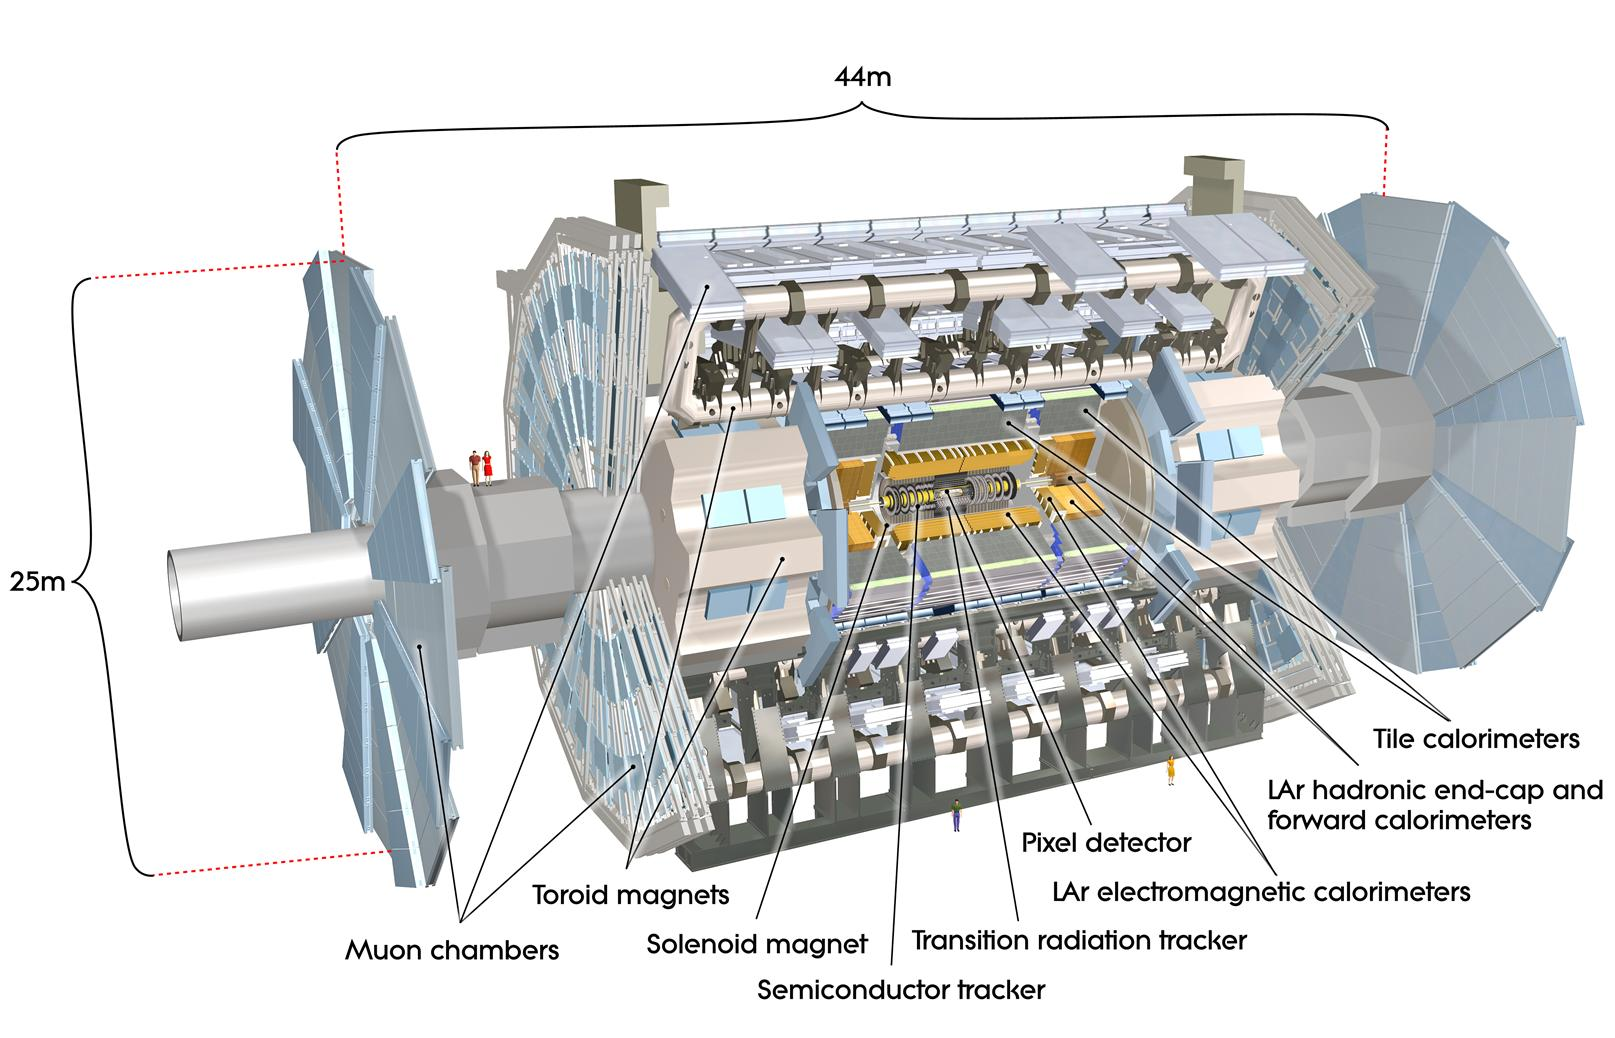
\includegraphics[scale=0.3]{ATLAS.jpg}
\caption{Cut-away view of the ATLAS detector.}
\end{figure}
The whole detector is covered by a magnet system that produces the electromagnetic field needed for measurement of the particles momenta.
\\
Integrated with the detector components there are the trigger and data acquisition system, a computing system which selects physics events with distinguishing characteristics and process them to extrapolate selected data.
\\
Being designed for general purposes, the detector must have a structure that allows to investigate a wide range of pyhsics, from the Higgs boson's analysis, to Standard Model measurements and future researches.

\section{The Inner Detector}
The ATLAS Inner Detector (ID)\cite{Aad:2010bx} is the first sub-detector which particles arising from the interaction find, just after the collision point. The detector is composed by a barrel and two end-cap regions to maximise the acquisition coverage, extending the pseudo-rapidity range up to $|\eta| < 2.5$ for particles coming from the LHC beam-interaction region, with full coverage in $\phi$. It is immersed in a 2 T magnetic field provided by a solenoid. Tracks measurements require a reasonably high resolution in the detection of the momentum of the particles and the multy-technology and high granularity of the Inner Detector increase the value of this parameter up to $\sigma_{p_T} / p_T = 0.05\%_{p_T} \text{GeV}$.
\\\\
Due to the extreme proximity at the interaction point, the ID design requires a high radiation resistance for all of its components and it is designed to detect particles using a series of different layers, as it can be seen in the split-view of Figure \ref{split-view}.
\\\\
\phantom{1}\hspace{0.3cm}The \emph{Pixel Detector} is the first sub-detector crossed by the particles produced in the interaction event. It is the real core in track reconstructing, because of its extremely high spatial resolution performance. The Pixel Detector consists of 1744 silicon pixel modules\cite{Aad_2008} arranged in three concentric barrel layers, positioned at radial dinstances of 50.5, 88.5 and 122.5 mm from the beam pipe, and two end-caps of three disks each, arranged at radial distances of 49.5, 58.0 and 65.0 mm respectively. The single module covers an active area of 16.4 mm $\times$ 60.8 mm and containts 47 232 pixels, most of size 50 $\mu$m $\times$ 400 $\mu$m.
\vspace{0.5cm}
\begin{figure}[t]
\centering
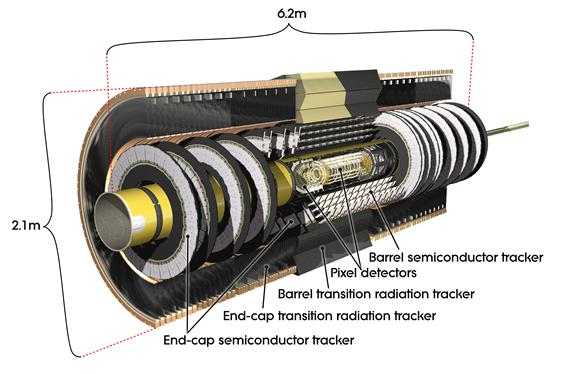
\includegraphics[scale=0.42]{inner_detector.jpg}
\caption{Split-view of the ATLAS Inner Detector}
\label{split_view}
\end{figure}
\\A module is read out by 16 radiation-hard front-end chips\cite{PERIC2006178} bonded to each sensor, so the total number of readout channels are $\sim$ 80.4 million. Hits in a pixel are read out if the signal exceeds a tunable threshold. Each particle crossing event defines tipically three measurement points for particles originating in the beam-interaction region.
\\
Between LHC Run1 and Run2 a fourth layer, konw as Insertiable B-Layer (IBL)\cite{Capeansjnh} has been installed between a new smaller beam pipe\footnote{The beam pipe diameter has been downcreased from 59 mm to 47 mm.} and the innermost layer (B-Layer) of the original Pixel Detector. This insertion in the tracking apparatus, so close to the interaction point, allowed to improve the quality of impact parameter reconstruction for tracks and thereby improving vertexing and $b$ tagging performance.
\\\\
\phantom{1}\hspace{0.3cm}The \emph{SemiConductor Tracker} (SCT) \cite{ABDESSELAM2006642, ABDESSELAM2007353} stands at the second stage of the particle tracking process, started with the Pixel Detector. It consists of 4088 modules of silicon-strip detectors arranged in four concentric barrels and two end-caps of nine disks each. In this way, as well as for the Inner Detector, the SemiConductor Tracker provides four more space points, placed at around 30, 37, 44 and 51 cm from the interaction point, bringing to eight the total number of space points for each particle's track. The intrinsic hit resolution of the SemiConductor Detector is a bit lower than for the Pixel Detector and it gets to $\sim 16 \mu$m along R-$\phi$ plane and $\sim 580 \mu$m along the z axis.
\\
Most modules consist of four silicon-strip sensors\cite{AHMAD200798} where two sensors on each side are chained together to give 768 strips of approximately 12 cm in length. A second pair of identical sensors is glued back-to-back with the first pair at a stereoangle of 40 mrad to provide space points. Since the detector is designed to perform tracking measurements, the hit informations gotten from an event is binary: once a particle hits the sub-detector, that will be registered only if the pulse height in a channel exceeds a preset threshold, normallycorresponding to a charge of 1 fC.
\\\\
\phantom{1}\hspace{0.3cm}The \emph{Transition Radiation Tracker} (TRT)\cite{collaboration_2008_TRT_barrel, collaboration_2008_TRT_endcaps} is the outer part of the tracking apparatus and covers radial distances from 563 mm to 1066 mm from the interaction point. It provides up to 36 additional space points to reconstruct the particles tracks, but the other side of the coin is its worst intrinsic spatial resolution of $\sim 130 \mu$m in the r-$\phi$ plane. The Transition Radiation Tracker is made of 298 304 proportional drift tubes, usually known as straws, with 4 mm in diameter, read out by 350 848 channels of electronics.The straws in the barrel region are arranged in three cylindrical layers and 32 $\phi$ sectors, while the straws in the endcap regions are radially oriented and arranged in 80 wheel-like modular structures.
\begin{figure}[h]
\centering
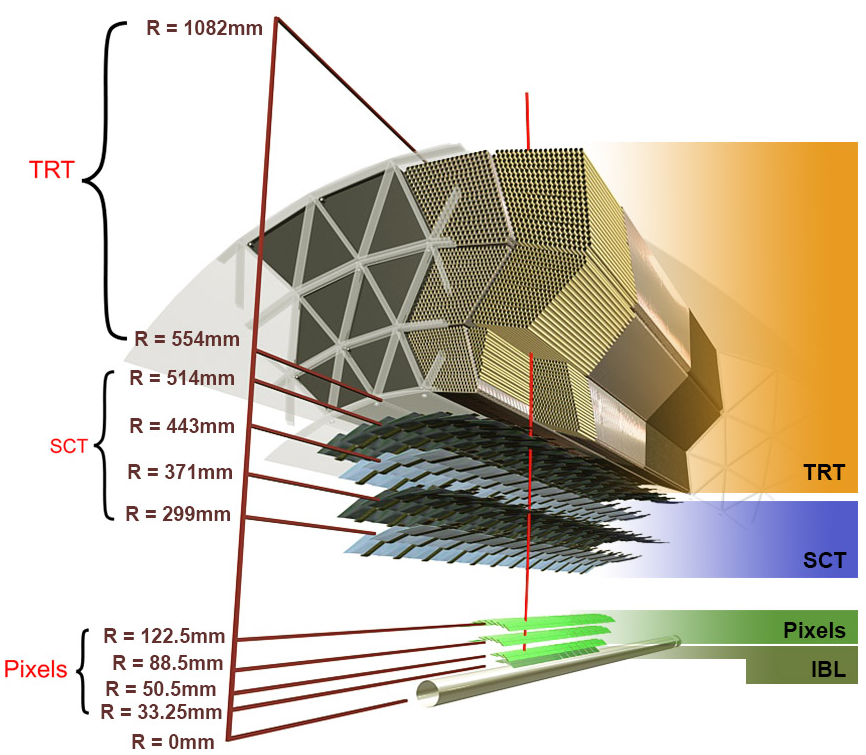
\includegraphics[scale=0.8]{split_view_ID.png}
\caption{Schematic view of the Inner Detector (ID) detailed layout, including the new Insertable B-Layer (IBL).}
\end{figure}
\\This kind of sub-detector works both as drift chamber measuring the charge drift time and as transition radiation detector to identify electrons by means of polypropylene fibres for the barrel or foils for the endcaps interleaved between the straws. The design of TRT allows charged particles with transverse momentum $pT>0.5$ GeV and with pseudo-rapidity of $|\eta| < 2.0$ to cross typically more than 30 straws.
\\\phantom{1}\hspace{0.3cm}The \emph{Cooling System} is designed to span a very wide range of temperatures, due to the peculiar operating environment for each sub-detector of the Inner Detector. The silicon detectors are cooled with a bi-phase evaporative system using C$_3$F$_8$ fluid at -25 \textdegree{}C. The target temperature for the silicon sensors is 0 \textdegree{}C for the Pixel Detector and -7 \textdegree{}C per the SemiConductor Tracker. These values were chosen to break down the radiation damages to the electronic systems.
\\\\
The overall Inner Detector relative momentum resolution before the IBL insertion 
\begin{equation}
\sigma_p / p = (4.83 \pm 0.16) \times 10^{-4}\text{GeV}^{-1} \times p_T
\end{equation}
has been measured for high momentum tracks.
\\
Since the amount of material to achieve the high granularity set in the Inner Detector, including read-out, cooling systems and supports, is quite sizable, some of the photons arising from the collision event may convert into electron-positron pairs before reaching the Electromagnetic Calorimeter as well as electrons may loose part of their energy through bremsstrahlung emissions. These kind of losses generally affect the energy resolution of the calorimeter system.

\section{The ATLAS calorimeters}
The ATLAS calorimeters system consists of three different types of sampling calorimeters, each of them designed to detect a precise family of particles. Typically the detection of photons and light particle electromagnetically interacting, such as electrons, is left to the Electromagnetic Calorimeter (ECal), covering the pseudorapidity region $|\eta| < 3.2$, while for hadrons the Hadronic Calorimeter (HCal) is preferred, with a pseudorapidity region of $|\eta| < 3.9$. To seal the system and to maximise the detection region, two Forward Calorimeters are sited at either end of the main barrel, to cover the pseudorapidity range of $3.1 < |\eta| < 4.9$ .
\\
The Calorimetric system have the main purpose of detecting particles by measuring the energy and the direction of incoming electrons, photons and hadrons, giving a fundamental contribution in the missing transverse energy measurement too.
\\
It consists of Sampling Calorimeters, where the absorbing material which degrades the energy of the particles and the active material that provides a measurable signal are alternated within the detector's volume. For ATLAS experiment calorimeters, Liquid Argon (LAr) or polystirene scintillator are used as active material, while lead (Pb), copper or iron are used as passive material.
\\
Passing through these layers, particles interact with the material producing showers whose energy and trajectory are measured. Depending on the nature of the incoming particle, it may start an electromagnetic shower, mainly detected in the electromagnetic calorimeter, or an hadronic shower, visible in the hadronic calorimeter.
\begin{figure}[h]
\centering
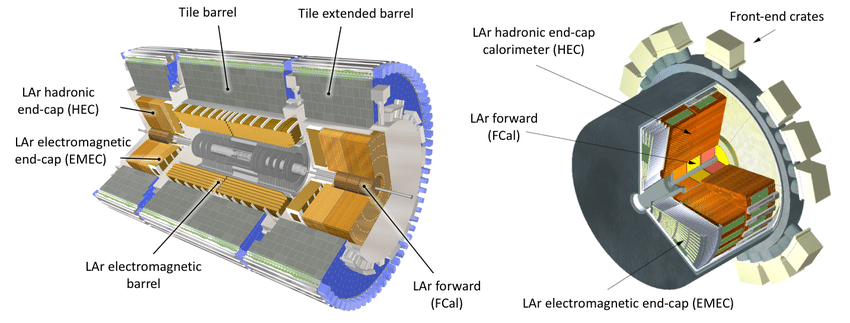
\includegraphics[scale=0.43]{calorimeters.png}
\caption{Subsystems of the ATLAS calorimeters and an enlarged view of the end-cap calorimeters.}
\end{figure}
\subsection{Electromagnetic showers}
At high energy, photons in matter convert into an electron-positron pair which then emit energetic bremsstrahlung photons. These, in turn, convert into further electron-positron pairs and so on. This chain reaction continue until the energy of the pair-produced electrons and positrons drops below an energy threshold, known as the \emph{critical energy} ($E_c$). Once that point is reached, the $e^+ e^-$ pairs will prefer atomic collisions rather than bremsstrahlung emission as energy loosing choice and breaking the cascade\cite{Leo302344}.
\\
The longitudinal development of the shower is governed by the \emph{Radiation Length} ($X_0$), defined as the amount of material which causes the electron to reduce its energy by a factor of $e$ \footnote{For Liquid Argon (LAr) and Lead (Pb), the critical energy and radiation length are
\begin{align*}
E_c^{LAr} = 32.84 \text{MeV} \hspace{0.2cm},& \hspace{0.4cm} X_0^{LAr} = 14 \text{cm} \\
E_c^{Pb} = 7.43 \text{MeV} \hspace{0.2cm},& \hspace{0.4cm} X_0^{Pb} = 0.56 \text{cm}
\end{align*}
Considering now an electron with an initial energy of $E_0 = 100 \text{GeV}$, the shower depth in LAr and Pb will be
\begin{align*}
L^{LAr}(95\%) &\sim 260 \text{cm} \\
L^{Pb}(95\%) &\sim 15 \text{cm}
\end{align*}}.
Considering $X_0$ related to the typical path necessary for a photon to create an $e^+e^-$ pair, the total number of particles in the shower after $t$ times $X_0$ turns out to be
\begin{equation}
N(t) = 2^t
\end{equation}
with an approximate energy for the single particle of
\begin{equation}
E(t)/\text{particle} = E_0/2^t
\end{equation}
Once the critical energy $E_c$ is reached, the shower stops and the maximum number of expected particles in the cascade can be calculated as
\begin{equation}
N_{max} \sim E_0 / E_c \hspace{0.2cm} \text{.}
\end{equation}
All of these parameters strictly depend on the atomic number Z of the detector material: in high-Z materials, particle multiplication continues longer and decreases more slowly than in low-Z materials or number of positrons strongly increases with the Z value of the absorber material.
\\
The critical energy $E_c$ is parametrized for liquid and solid materials as:
\begin{equation}
E_c = \frac{610 \text{MeV}}{Z+1.24}
\end{equation} 
where Z is the atomic number of the material, while the \emph{radiation length} ($X_0$) is definded as
\begin{equation}
X_0 = \frac{716.4[\text{g}\hspace{0.05cm}\text{cm}^{-2}] \times A}{Z(z+1)\ln(287/\sqrt{Z})} \hspace{0.2cm} \text{.}
\end{equation}
The material thickness needed to contain the 95 \% of the longitudinal energy profile of the shower is the \emph{shower depth}
\begin{equation}
L(95\%) \sim t_{max} + 0.08Z + 9.6 = \Bigl[\ln\Bigl(\frac{E_0}{E_c}\Bigr) + C_j \Bigr] + 0.08Z + 9.6 \hspace{0.5cm} [X_0]
\end{equation}
where $E_0$ is the energy of the incoming particle and $C_j$ is a parameter which can be $-0.5$ or $+0.5$ depending on the incident particle being an electron or a photon respectively. It is expressed in units of $X_0$.
\\\\
The last important parameter for electron and photon shower is the \emph{Moliere radius} ($R_M$), which is related to the lateral development of the shower and it is defined as
\begin{equation}
R_M = \frac{21 \text{MeV}}{E_c}X_0 \hspace{0.2cm} \text{.}
\end{equation}
Up to 95\% of an electromagnetic shower is enclosed in twice the $R_M$.

\subsection{Hadronic showers}
Considerably different from electrons and photons with electromagnetic showers, hadrons produce a shower of secondary particles, known as hadronic showers, within which two different kinds of processes are involved.
\begin{itemize}
\item The electromagnetic component represent up to 30-60\% of the total energy and it derives from $\pi^0$ pions decays into two collimated photons.
\item The hadronic component leads the main contribution at the shower generation combining several processes, such as slow neutrons production or spallation protons. Part of the energy released in the hadronic calorimeter does not contribute to the signal. This kind of invisible energy is due to the nucleons released in the nuclear reactions and represents up to 40\% of the total amount of energy liberated.
\end{itemize}
The main parameter which describes the hadronic showers is the \emph{nuclear interaction length} $\lambda_{int}$, representing the average distance a high-energy hadron has to travel inside a medium before a nuclear interaction occurs, is described as
\begin{equation}
\lambda_{int} \sim 35 A^{1/3} \text{g cm}^{-2} \hspace{0.2cm} \text{.}
\end{equation}
Similarly to the shower depth for electromagnetic showers, 95\% of the longitudinal energy deposit profile of the hadronic shower is contained in
\begin{equation}
t_{95\%} = t_{max} + 2\lambda E^{0.13}
\end{equation}
where $t_{max}$ is
\begin{equation}
t_{max} = 0.2\ln(E/1 \text{GeV}) + 0.7 \hspace{0.5cm} [\lambda]
\end{equation}
expressed in units of nuclear interaction length\footnote{Considering Liquid Argon (LAr) and Lead (Pb) and an incoming pion with $E_{\pi} = 100 \text{GeV}$, the values for $\lambda_{int}$ and $t_{95\%}$ are
\begin{align*}
\lambda_{LAr} = 85.77 \text{cm} \hspace{0.2cm} &, \hspace{0.4cm} t_{95\%}^{LAr} = 450 \text{cm} \\
\lambda_{LAr} = 85.77 \text{cm} \hspace{0.2cm} &, \hspace{0.4cm} t_{95\%}^{LAr} = 450 \text{cm} \hspace{0.2cm} \text{.}
\end{align*}}.
\\
Since $\lambda$ is much larger than the radiation length $X_0$, a considerable thicker detector\footnote{To contain a 100 GeV pion, a layer of Lead almost 6 times thicker than the one requested to contain a same-energy electron is needed.}. Therefore, in the experiment design usually electromagnetic calorimeters fit before the hadronic calorimeters.

\subsection{The ATLAS Electromagnetic Calorimeter}
The ATLAS Electromagnetic Calorimeter (ECal)\cite{CERN-LHCC-96-041, Aad2010ai} is composed of a central barrel region, which covers $|\eta| < 1.4$, and two end-caps to extend the $\eta$ region to $1.4 < |\eta| < 3.2$. It is a sampling calorimeter consisting of two half-barrels, centered around the ATLAS beam axis (typically the $z$-axis), where one of these half-barrels covers $z > 0$ and pseudorapidity $\eta > 0$ and the other covers $z < 0$ and pseudorapidity $\eta < 0$. The calorimeter itself is made of several 2 mm layers of Liquid Argon as active medium spaced out by Lead absorber plates with different thickness for $|\eta| < 0.8$ and $|\eta| > 0.8$\footnote{The Lead absorber plates have a thickness of 1.5 mm for $|\eta| < 0.8$, while 1.3 mm for $|\eta| > 0.8$.}
, glued between two 0.2 mm thick stainless steel sheet, in order to improve their mechanical strength. For ease of construction, both half-barrels are divided into 16 modules, each with a thickness of at least 22 radiation lengths ($X_0$), increasing from 22$X_0$ to 30$X_0$ between $|\eta| = 0$ and $|\eta| = 0.8$, and from 24$X_0$ to $33X_0$ between $|\eta = 0.8$ and $|\eta = 1.3$.
\\
Once assembled, active materials and absorbers are arranged into an accoridon-shape structure, leaving no discontinuity along the azimuthal angle $\phi$ and avoiding cracks due to the outgoing read-out system.
\\\\
The 275 $\mu$m read-out electrodes consist of three conductiove copper layers separated by insulating polymide sheets. The two outer layers are at the high voltage potential, while the inner one is used for reading out the signal through capacitive coupling.
\begin{figure}[h]
\centering
\subfloat{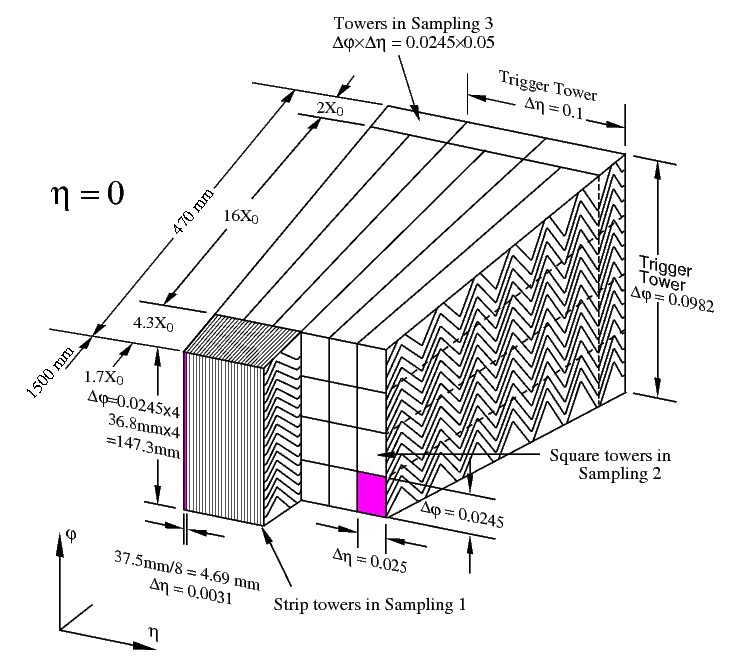
\includegraphics[scale=0.25]{calorimeter_sketch.png}}
\subfloat{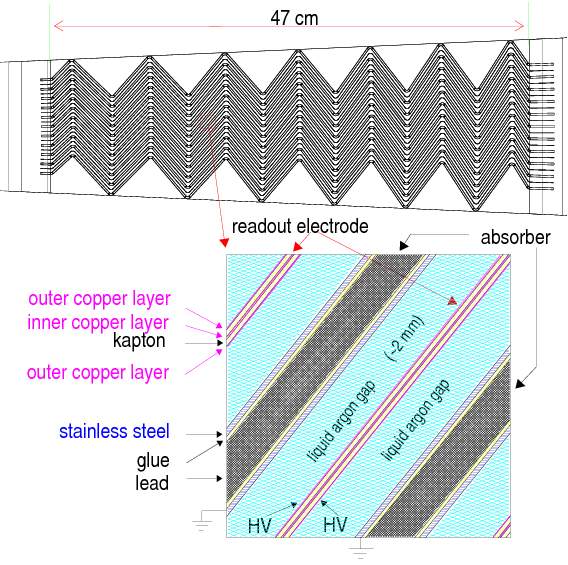
\includegraphics[scale=0.3]{accordion_structure.png}}
\caption{Sketch of a LAr calorimeter barrel module with a focus on the accordion structure and its layers granularity in $\eta$ and $\phi$.}
\end{figure}
\phantom{i}
\\To improve the precision in the recording of the longitudinal development of the electromagnetic showers, the Electromagnetic Calorimeter is segmented into four different longitudinal layers:
\begin{itemize}
\item The \emph{Presampler} (PS) is the innermost and thinnest layer of the system, with a thickness of 1.1 cm only and it is placed inside the solenoid, covering the $|\eta| < 1.8$ region. It is a single layer of Liquid Argon, but with no Lead absorber in front and it has been designed to correct for the energy loss in the Inner Detector, solenoid and cryostat wall;
\item The \emph{Layer 1} (L1) has a depth of 6 radiation lengths, including the material in front. This layer has the finest segmentation along $\eta$ with each strip of size $(\Delta \eta \times \Delta \phi) = (0.0031 \times 0.1)$, providing an excellent resolution in the $\eta$ coordinate in order to discriminate between photons related with the selected event and  $\pi^0$ decaying in two collinear photons;
\item The \emph{Layer 2} (L2) is where most of the energy is deposited and it extends the depth up to 22 radiation lengths. Clusters with energy below 50 GeV are generally fully contained in the Layer 2\footnote{Typically, the majoirty of the energy for showers generated by electrons or photons with energy up to 50 GeV is released in the 16 radiation lengths region.}. For the position measurement of the cluster, in this layer both $\eta$- and $\phi$-coordinates are equally important and therefore it is segmented into square cells of size $(\Delta \eta \times \Delta \phi) = (0.025 \times 0.025)$;
\item The \emph{Layer 3} (L3) completes the calorimeter layers, adding two more radiation lengths in the apparatus. Only the highest-energy electrons and photons can reach this deep in the detector in wide showers by now. For this reason the cell size in this layer can be doubled in the $\eta$ direction without loss of resolution. It is used to estimate the energy losses in the Hadronic Calorimeter placed right after.
\end{itemize}
In the end-cap there is less material in front of the calorimeter and the presampler can be avoided for $|\eta| > 1.81$. The end-caps start at $|\eta| = 1.5$ and continue down to $|\eta| = 3.2$ but with an increased cell size above $|\eta| = 2.5$ . The most critical point in the calorimetric apparatus is where the end-cap and barrel calorimeters meet. In this point there is a crack with bad energy resolution, but a large effort has gone into reducing the size of the crack while still leaving space for cables and cooling for the Inner Detector.
\\
The nominal Electromagnetic Calorimeter resolution is parametrized as
\begin{equation}
\frac{\Delta E}{E} = \frac{a}{\sqrt{E}} \oplus \frac{b}{\sqrt{E}} \oplus c \hspace{0.2cm} \text{.}
\end{equation}
The sampling term $a$, also known as \emph{stochastic term}, is defined by the number of lead/argon interfaces. The term $b$ includes the contribution arising from the electronic noise, typically negligible in the energy range studied in the ATLAS experiment. The last term $c$ is called \emph{constant term} and affects the resolution for high-energy clusters. It is limited by alignment, electronic calibration uncertainties and global detector non-uniformities.
\\
The resolution is estimated to be
\begin{equation}
\frac{\sigma(E)}{E} \approx \frac{(10\% \div 17\%)}{\sqrt{E}} \oplus 0.7\%
\end{equation}

\subsection{The ATLAS Hadronic Calorimeter}
The Hadronic Calorimeter (HCal)\cite{ATLAS1996aa, Aad2010af}, or Tile Calorimeter, is a large hadronic sampling calorimeter where iron and scintillating plates read-out by wavelength shifting (WLS) fibres are used as the absorber material and as active medium respectively. The highly periodic structure of the calorimeter allows the division of the whole detector into sub-modules, as shown in Fig.\ref{TiLe_modules}. A good sampling homogeneity is obtained when the calorimeter is placed behind an electromagnetic compartiment and a coil equivalent to a total of about two nuclear interaction lengths ($\lambda_{int}$) of material.
\\
The calorimeter consists of a long cylindrical structure with inner and outer radius of 2.28 m and 4.23 m respectively, divided into a 56.40 m long central barrel and two 29.10 m extended-barrels (Fig.\ref{TiLe_modules}), covering the pseudorapidity region $|\eta| < 3.9$ in total. The central barrel region is divided in cells of size $(\Delta \eta \times \Delta \phi) = (0.1 \times 0.1)$ and covers the pseudorapidity region $|\eta| < 1.7$, while in the end-cap sections the granularity changes from $(\Delta \eta \times \Delta \phi) = (0.1 \times 0.1)$ to $(\Delta \eta \times \Delta \phi) = (0.2 \times 0.2)$ depending on $\eta$, using Liquid Argon as active material and copper and tungsten plates as absorbers.
\\
Similarly to the Electromagnetic Calorimeter, the Tile Calorimeter must be several nuclear interaction lengths $\lambda$ thick to ensure all the hadronic clusters is blocked and consequently all the energy is collected. For that reason around 11 nuclear interaction lengths are covered at the outer radius.
\\
The nominal energy resolution for hadronic jets, combined with electromagnetic calorimeter's informations, is
\begin{equation}
\frac{\sigma(E)}{E} \approx \frac{50\%}{\sqrt{E}} \oplus 3\%
\end{equation}
\begin{figure}[h]
\centering
\subfloat[][]{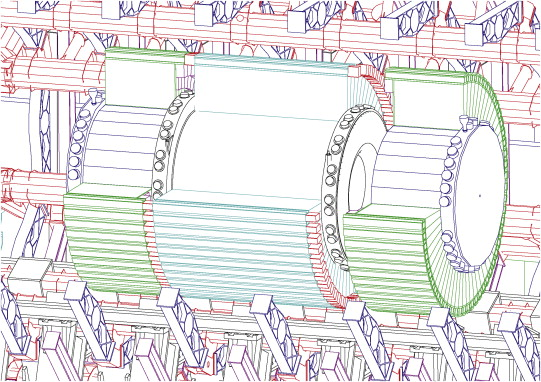
\includegraphics[scale=0.51]{tile_calorimeter.png}} \hspace{0.5cm}
\subfloat[][]{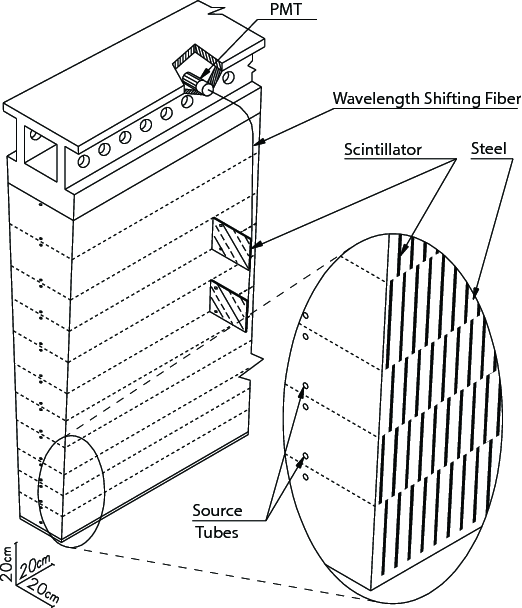
\includegraphics[scale=0.21]{TileCal_Module.png}}
\caption{a)Split figure of Tile Calorimeter, showing both the barrel and two extended barrel sections; b)Mechanical structure of a calorimeter's module.}
\label{TiLe_modules}
\end{figure}

\subsection{The Forward Calorimeter}
The Forward Calorimeter (FCal) \cite{Artamonov_2008}, placed near the incident beams at 4.7 m from the interaction point, complete the nearly $4\pi$ sterad coverage for high $p_T$ particles resulting from proton-proton collisions in the ATLAS detector.
\\
The Forward Calorimeter covers the pseudorapidity range $3.1 < |\eta| < 4.9$ and provides measurements of both electromagnetic and hadronic showers. For this purpose this calorimeter is segmented into different parts, each of them expecially designed for the one or the other shower. In particular, the electromagnetic segment uses Copper as absorber material and Liquid Argon (LAr) as active medium, while the hadronic segment is made of Tungsten as absorber, letting the Liquid Argon as sensitive material.
\\
Since the FCal is placed so close to the incident beams, the jets seen in the detector typically are of high energy. For that reason, the effective energy resolution, parametrized as \cite{Archambault_calibration}
\begin{equation}
\frac{\sigma_E}{E} = \frac{a}{\sqrt{E}} \oplus c
\end{equation}
is dominated by the constant term, where
\begin{equation}
\frac{\sigma_E}{E} = \frac{(28.5 \pm 1.0)\%}{\sqrt{E}} \oplus (3.5 \pm 0.1)\%
\end{equation}
was measured for electrons and
\begin{equation}
\frac{\sigma_E}{E} = \frac{(94.2 \pm 1.6)\%}{\sqrt{E}} \oplus (7.5 \pm 0.4)\%
\end{equation}
for pions, between 20GeV and 200 GeV.
\\
In order to study the longitudinal shower development, the FCal is divided into three different sections, visible in Fig.\ref{FCal}. In all of the three sections only radiation hard materials are used, and there are no adhesive used in joints. FCal1 is designed to detect electromagnetic showers, while FCal2 and FCal3 are denser and serve to stop and collect the energy released in the hadronic showers.
\begin{figure}[h]
\centering
\subfloat{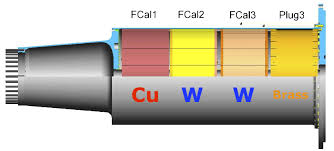
\includegraphics[scale=0.55]{atlas_fcal.jpeg}}
\subfloat{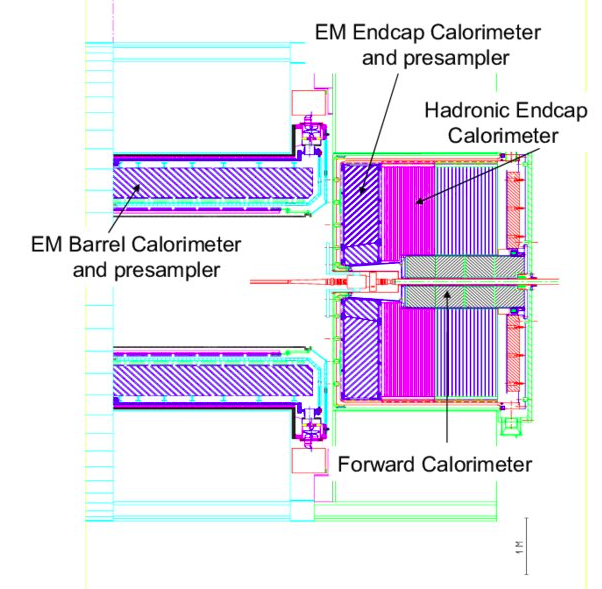
\includegraphics[scale=0.2]{fcal_position.png}}
\caption{The general arrangement of the Forward Calorimeter.}
\label{FCal}
\end{figure}

\section{The Muon Spectrometer}
Most of the particles produced in a collision are absorbed by either electromagnetic or hadronic calorimeter. The only particles which exceed all the layers of the detector are neutrinos and muons. If the only way to detect neutrinos is the missing energy's analysis because they don't interact with any of the layers, muons are detected by the Muon Spectrometer (MS) \cite{CERN-LHCC-97-022}, the last ATLAS layer.
\\\\
The purpose of this detector is the high-precision measurement of the muon momentum, involving the magnetic deflection of the muon tracks, caused by the toroidal magnetic field. The Muon Spectrometer is divided into three parts, a central barrel closed by two end-caps, covering the pseudorapidity range $|\eta| < 2.7$, except for a small region $|\eta| < 0.1$ needed by the services for the inner detectors. In the region $1.0 < |\eta| < 1.4$, referred to as transition region, the magnetic deflection is provided by a combination of barrel and end-cap fields, making the field mostly orthogonal to the muon trajectories.
\\\\
The muon trajectories are bended by the magnetic field in the ($R$, $z$) plane, using two different systems to measure the hits. In the barrel region, tracks are measured in three cylindrical chambers concentric with the beam axis, while in the transition and end-cap regions the three chambers are installed vertically. Different types of detectors are used in the various regions: Monitored Drift Tubes (MDTs) in the barrel cover $|\eta| < 2.7$ and Cathode Strip Chambers (CSCs) in the forward region cover $2.0 < |\eta| < 2.7$.
\\
Each MDT's chamber is made of 3-8 layers of drift tubes filled with a non-flammable Ar-CH$_4$-N$_2$ at 3 bar absolute pressure and with an average single-wire resolution of 80 $\mu$m and 35 $\mu$m per chamber. The tube lengths vary from 70 cm to 630 cm.
\vspace{0.5cm}
\begin{figure}[b!]
\centering
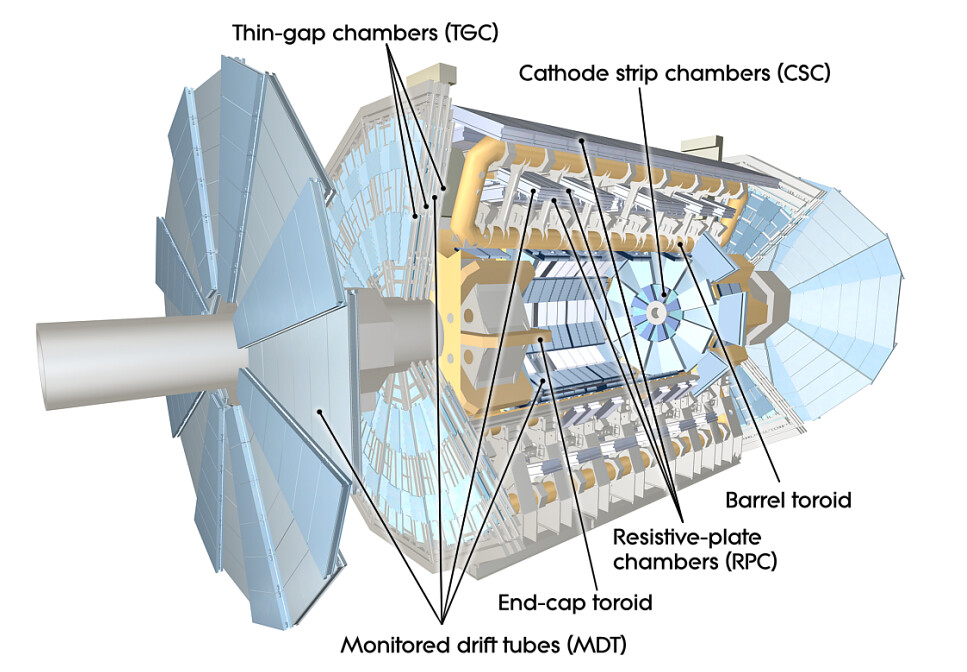
\includegraphics[scale=0.45]{muon_spectrometer.jpg}
\caption{Cut view of the Muon Spectrometer system.}
\end{figure}
\\The Cathode Strip Chambers, differently from MDTs, are multiwire proportional chambers optimized to have the wires oriented in the radial direction. The precision coordinate is obtained by measuring the charge induced on the segmented cathode by the avalanche formed on the anode wire. This design allows to have a resolution of 60 $\mu$m in the bending plane and 4 mm in the transverse plane. Other important characteristics are small electron drift times ($\leq 30$ ns), good time resolution (7 ns), good two-tracks resolution and low neutron sensitivity.
\\\\
The ATLAS Muon Spectrometer system, in particular the Monitored Drift Tubes, provides a momentum resolution between 2-3\% an $\sim$10\% in a $p_T$ range between 10 GeV and 1 TeV. 